In order to minimize the burden of processing on the individual clients that utilize our system the application takes a lightweight-client approach to the traditional client-server application.

\begin{figure}[h!]
	\centering
 	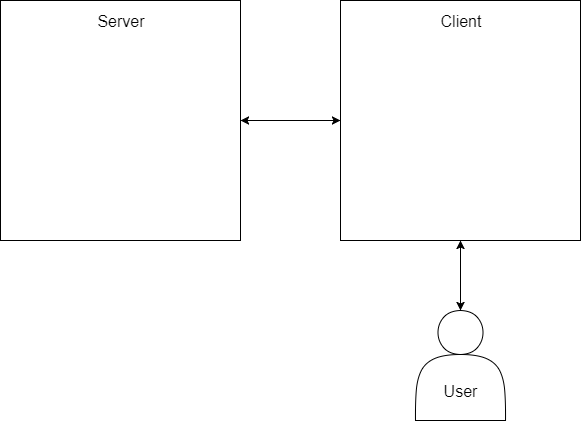
\includegraphics[width=0.60\textwidth]{images/layers}
 \caption{A high-level data-flow diagram for our application}
\end{figure}

\subsection{Client Layer}
The client will function as the HMI between our system and the user. It consists of a UI, and methods by which it may communicate with the server.

\subsection{Server Layer}
The server will function as the work-horse for the application. It's purpose is to host the visualization function which will map an input of word, audio to a distance metric in the form of x, y co-ordinates.
